\documentclass[a4paper,12pt]{article}

%\usepackage[latin1]{inputenc}
\usepackage{amsfonts}
\usepackage{amsmath}
\usepackage{amssymb}
\usepackage{amsthm}
\usepackage{color}
\usepackage[ngerman]{babel}
\usepackage[pdftex]{graphicx}
%\usepackage[T1]{fontenc}
\usepackage{gauss}

\pagestyle{empty}
\usepackage[utf8]{inputenc}
\usepackage{listings}
\definecolor{Brown}{cmyk}{0,0.81,1,0.60}
\definecolor{OliveGreen}{cmyk}{0.64,0,0.95,0.40}
\definecolor{CadetBlue}{cmyk}{0.62,0.57,0.23,0}
\definecolor{lightlightgray}{gray}{0.9}
\lstset{
    language=C,                             % Code langugage
    basicstyle=\rm\ttfamily,                % Code font, Examples: \footnotesize, \ttfamily
    keywordstyle=\color{OliveGreen},        % Keywords font ('*' = uppercase)
    commentstyle=\color{gray},              % Comments font
    numbers=left,                           % Line nums position
    numberstyle=\tiny,                      % Line-numbers fonts
    stepnumber=1,                           % Step between two line-numbers
    numbersep=5pt,                          % How far are line-numbers from code
    backgroundcolor=\color{lightlightgray}, % Choose background color
    frame=none,                             % A frame around the code
    tabsize=2,                              % Default tab size
    captionpos=b,                           % Caption-position = bottom
    breaklines=true,                        % Automatic line breaking?
    breakatwhitespace=false,                % Automatic breaks only at whitespace?
    showspaces=false,                       % Dont make spaces visible
    showtabs=false,                         % Dont make tabls visible
    %columns=flexible,                       % Column format
    %morekeywords={someword, otherword},     % specific keywords
}



%\topmargin20mm
\oddsidemargin0mm
\parindent0mm
\parskip2mm
\textheight24cm
\textwidth15.8cm
\unitlength1mm
\usepackage{pdfpages}

\begin{document}




{\bf Aufgabe 1: Kombinatorik}

Sie geben eine Party und laden 10 Leute ein.

{\bf a) }

Wie viele Möglichkeiten gibt es, die 10 Gäste an einen Tisch mit 10 Stühlen zu setzen?

{\bf b)}

 Jeder Gast soll mit jedem anderen Gast anstoßen. Wie oft klirren die Gläser?

\hspace{10mm}



{\bf Aufgabe 2: Bedingte Wahrscheinlichkeiten}

In einer Fabrik werden die produzierten Werkstücke vor der Auslieferung überprüft. Hierfür werden für jedes Werkstück  hintereinander zwei Funktionstest durchgeführt.  Die Wahrscheinlichkeit, dass ein Werkstück beide Tests besteht, betrage $0.5$. Die Wahrscheinlichkeit, dass ein Werkstück  den ersten Test besteht betrage $0.6$. 

{\bf a) }

Berechnen Sie die Wahrscheinlichkeit, dass ein Werkstück den zweiten Test besteht, wenn er bereits den ersten bestanden hat.

{\bf b) }

Angenommen, die beiden Tests sind stochastisch unabhängig. Wie hoch ist dann die Wahrscheinlichkeit, dass ein Werkstück den zweiten Test besteht?

\hspace{10mm}

{\bf Aufgabe 3: Wahrscheinlichkeitsraum und Verteilungen}

{\bf a)  }

Was versteht man unter einem Laplace-Experiment?

{\bf b) }

Geben Sie eine Konstante $c  \in \mathbb{R}$ an, so dass die Funktion 
\begin{align*}
f(x) = \begin{cases} c x^3 \text{ für }  0\leq x \leq 2 \\ 0 \text{ sonst}\end{cases}
\end{align*}
ein Dichte auf $\mathbb{R}$ definiert.

\hspace{10mm}


{\bf Aufgabe 4: Zufallsvariablen und Erwartungswert}

{\bf a)}

Die Zufallsvariablen $X_1$ und $X_2$ seien stochastisch unabhängig   und im Intervall $[0,2]$ gleichverteilt.
Berechnen Sie den Erwartungswert der Zufallsvariablen $Y = 2 \cdot X_1 \cdot X_2 + X_1^2$.

{\bf b) }

Erklären Sie die Aussage des zentralen Grenzwertsatzes anhand eines Beispiels.


\newpage

{\bf Aufgabe 5: Hypothesentest }

In den Nachrichten sehen Sie, dass  es im sonnigen Schwetzingen im Schnitt an höchstens  20 von 100 Tagen regnet. Sie möchten diese Hypothese überprüfen und beobachten hierfür an $n=20$ Tagen das Wetter. Erstellen Sie einen geeigneten Hypothesentest. 
Wie sollte Ihre Entscheidungsregel dann lauten, wenn Sie sicherstellen möchten, dass die Hypothese mit einer Irrtumswahrscheinlichkeit von $0.025$ unberechtigter Weise abgelehnt wird.


\newpage
Verteilungsfunktion für die Binomialfunktion  $P(x \leq k ) =  \sum_{i=0}^k \begin{pmatrix} n \\ i \end{pmatrix} \rho^i (1-\rho)^{n-i}$ \\

%\includepdf[pages={4}, scale=0.75]{binomialverteilung_verteilungsfunktion.pdf}
\includegraphics[scale=0.5,page=4] {bv}

{\end{document}
